\documentclass[a4paper]{article}
% mathmatical fonts and formulations
\usepackage{amsfonts}
\usepackage{amsmath}
\usepackage{amsthm}
\usepackage{amssymb}
% float control
\usepackage{placeins}
% graphic control
\usepackage{pgf}
\usepackage{tikz}
\usepackage{xcolor}
% excercise
%\usepackage{exercise}
% Algorithm support
%\usepackage{algorithmic}
\usepackage{algorithm2e}
% Set space
\usepackage[top=1.54cm,bottom=1.54cm,left=3.18cm,right=2.54cm,includehead,includefoot
           ]{geometry}
%color of the word
\usepackage{color}
% change the counter of enumerate
\usepackage{enumerate}
% allow to use the block
\usepackage{framed}
% introduce indent at the beginning of every pragraph
\usepackage{indentfirst}
% every section begins at a new page
%\usepackage{titlesec}
\newcommand{\sectionbreak}{\clearpage}

\theoremstyle{definition}
\newtheorem{lemma}{Lemma}[section]
\newtheorem{theorem}{Theorem}[section]
\newtheorem{definition}{Definition}[section]
\newtheorem{corollary}{Corollary}[section]
\newtheorem{exercise}{Exercise}[section]
\newtheorem{example}{Example}[section]
\newtheorem{observe}{Observation}[section]

\date{}
\author{}
\title{COMP3721 Tutorial 4}

% set the way to number equation
\numberwithin{equation}{subsection}
%depth of table of contents
\setcounter{tocdepth}{2}
\begin{document}
\maketitle
\section{NFA $\rightarrow$ Regular Expression}

\begin{enumerate}[1.]
	\item Write regular expressions for the languages accepted by the following NFA.
	\begin{center}
		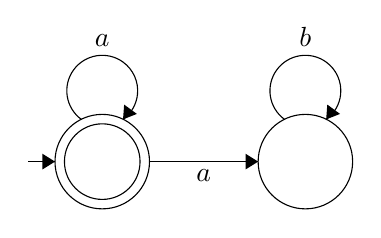
\begin{tikzpicture}[scale=0.2]
		\tikzstyle{every node}+=[inner sep=0pt]
		\draw [black] (14.1,-20.1) circle (3);
		\draw [black] (14.1,-20.1) circle (2.4);
		\draw [black] (27,-20.1) circle (3);
		\draw [black] (9.4,-20.1) -- (11.1,-20.1);
		\fill [black] (11.1,-20.1) -- (10.3,-19.6) -- (10.3,-20.6);
		\draw [black] (17.1,-20.1) -- (24,-20.1);
		\fill [black] (24,-20.1) -- (23.2,-19.6) -- (23.2,-20.6);
		\draw (20.55,-20.6) node [below] {$a$};
		\draw [black] (12.777,-17.42) arc (234:-54:2.25);
		\draw (14.1,-12.85) node [above] {$a$};
		\fill [black] (15.42,-17.42) -- (16.3,-17.07) -- (15.49,-16.48);
		\draw [black] (25.677,-17.42) arc (234:-54:2.25);
		\draw (27,-12.85) node [above] {$b$};
		\fill [black] (28.32,-17.42) -- (29.2,-17.07) -- (28.39,-16.48);
		\end{tikzpicture}
	\end{center}
	
	\begin{center}
		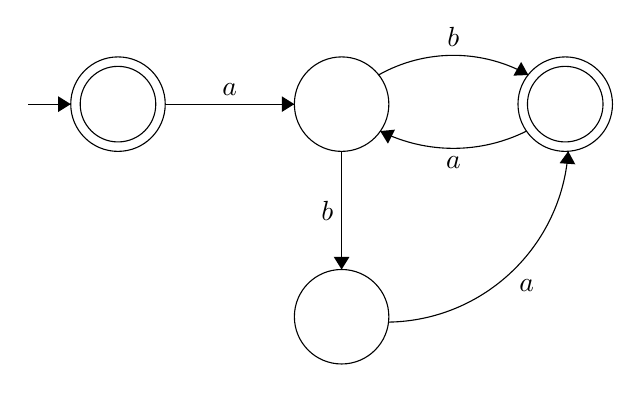
\begin{tikzpicture}[scale=0.2]
		\tikzstyle{every node}+=[inner sep=0pt]
		\draw [black] (16.9,-19.5) circle (3);
		\draw [black] (16.9,-19.5) circle (2.4);
		\draw [black] (31.1,-19.5) circle (3);
		\draw [black] (45.3,-19.5) circle (3);
		\draw [black] (45.3,-19.5) circle (2.4);
		\draw [black] (31.1,-33) circle (3);
		\draw [black] (11.2,-19.5) -- (13.9,-19.5);
		\fill [black] (13.9,-19.5) -- (13.1,-19) -- (13.1,-20);
		\draw [black] (19.9,-19.5) -- (28.1,-19.5);
		\fill [black] (28.1,-19.5) -- (27.3,-19) -- (27.3,-20);
		\draw (24,-19) node [above] {$a$};
		\draw [black] (33.445,-17.648) arc (119.42328:60.57672:9.68);
		\fill [black] (42.96,-17.65) -- (42.5,-16.82) -- (42.01,-17.69);
		\draw (38.2,-15.9) node [above] {$b$};
		\draw [black] (42.847,-21.209) arc (-63.40516:-116.59484:10.381);
		\fill [black] (33.55,-21.21) -- (34.04,-22.01) -- (34.49,-21.12);
		\draw (38.2,-22.81) node [below] {$a$};
		\draw [black] (31.1,-22.5) -- (31.1,-30);
		\fill [black] (31.1,-30) -- (31.6,-29.2) -- (30.6,-29.2);
		\draw (30.6,-26.25) node [left] {$b$};
		\draw [black] (45.49,-22.486) arc (-3.7482:-89.147:11.616);
		\fill [black] (45.49,-22.49) -- (44.94,-23.25) -- (45.94,-23.32);
		\draw (42.86,-30.63) node [below] {$a$};
		\end{tikzpicture}
	\end{center}
\end{enumerate}
\section{Application of Finite Automuta}
\begin{enumerate}[1.]
\item Prove that if $L$ is regular, then the following languages are also regular.
    \begin{enumerate}[(a)]
        \item $Subseq(L) = \{\textrm{$w_1\ldots w_k$ : $x = x_0w_1\ldots w_kx_k \in L$ for some $x_0,\ldots,x_k$}\}$.
        \item $L^R = \{\textrm{$w$ : $w^R\in L$}\}$.
    \end{enumerate}
\end{enumerate}
\section{Pumping Theorems}
\begin{enumerate}[1.]
\item Are the following languages on $\{a,b\}$ regular or not? Prove your answer.
    \begin{enumerate}[(a)]
        \item $\{\textrm{$a^ib^j$ : $i > j\geq 1$}\}$.
        \item $\{\textrm{$ww$ : $w\in \{a,b\}^*$}\}$.
        \item $\{\textrm{$(bab)^i(babbab)^i$ : $i\geq 1$}\}$.
    \end{enumerate}
\end{enumerate}
\section{More Problems}
\begin{enumerate}[1.]
\item Are the following statements true or false?
\begin{enumerate}[(a)]
\item Every subset of a regular language is regular.
\item If $L$ is regular, then so is $\{\textrm{$xy$ : $x\in L$ and $y\notin L$ }\}$.
\item $\{\textrm{$w$ : $w = w^R$}\}$ is regular.
\item If $L$ is a regular language, then so is $\{\textrm{$w$ : $w\in L$ and $w^R\in L$}\}$.
\end{enumerate}
\end{enumerate}
\end{document}

